\section{Results}
\label{sec:results}

\subsection{Primary outcomes: the convergence asymmetry}
\label{sec:results-primary}

Table~\ref{tab:primary-summary} summarizes the per-condition primary outcomes. At convergence, $\Delta_{\text{profit}}$ is comparable across conditions: $0.4932$ (95\% percentile bootstrap CI $[0.3494, 0.6369]$) at GATE-5, $0.4522$ (95\% CI $[0.3873, 0.5172]$) at GATE-2; both capture roughly half of the Nash-to-Monopoly profit gap. Convergence dynamics, however, differ sharply: GATE-5 reaches the pre-registered convergence criterion in $30/30$ repetitions ($100.0\%$) within the 50-round horizon, while GATE-2 reaches it in $1/15$ repetitions ($6.7\%$). The pre-registered Stage 3 go/no-go gate fires \textbf{PROCEED} for GATE-5 and \textbf{HALT} for GATE-2 on convergence-rate grounds. We read this comparable-$\Delta_{\text{profit}}$-but-divergent-convergence asymmetry mechanistically in \S\ref{sec:discussion-asymmetry} as evidence of a wider basin of attraction at smaller agent counts (mechanism refined to reading \emph{(a$'$)} in \S\ref{sec:discussion-asymmetry-cot} per the pre-registered Addendum \#5 and Addendum \#6 tests); the basin-width hypothesis and its Stage 3 falsification clause are pre-committed in \S\ref{sec:discussion-falsifiability}.

\begin{table}[h]
\centering
\caption{Primary outcomes per condition. $\Delta_{\text{profit}}$ at convergence is comparable across $n=5$ and $n=2$ ($0.49$ vs $0.45$, both $\approx \tfrac{1}{2}$ the Nash-to-Monopoly gap), but convergence rate within 50 rounds differs sharply ($100\%$ vs $6.7\%$) --- the asymmetry that anchors this paper.}
\label{tab:primary-summary}
\begin{tabular}{lcccccc}
\toprule
Condition & $n_{\text{rep}}$ & $\Delta_{\text{profit}}$ & 95\% CI & $p_{\text{high}}$ / $p_{\text{mid}}$ / $p_{\text{low}}$ & Converged & Stage 3 \\
\midrule
GATE-5 ($n = 5$) & 30 & 0.4932 & $[0.3494, 0.6369]$ & $0.267$ / $0.000$ / $0.733$ & 30/30 & PROCEED \\
GATE-2 ($n = 2$) & 15 & 0.4522 & $[0.3873, 0.5172]$ & $0.000$ / $0.267$ / $0.733$ & 1/15 & HALT \\
\bottomrule
\end{tabular}
\end{table}

For reference, $Q$-learner Bertrand experiments at matched logit-demand parameters \citep{calvano_etal_2020_ai_algorithmic_pricing_collusion} report terminal-price distributions concentrated in the upper half of the Nash--Monopoly range; our $\Delta_{\text{profit}} \approx 0.49$ at $n=5$ and $\approx 0.45$ at $n=2$ are accordingly partial-coordination outcomes, not $Q$-learner-equivalent supra-competitive outcomes. The cross-family contrast is the explicit subject of the Stage 4 design (\S\ref{sec:discussion-falsifiability}).

Parse-failure rates were $0.000\%$ across all $9000$ agent-round invocations in both conditions; the pre-registered $> 5\%$ post-round-25 stopping rule was not triggered.

\begin{figure}[h]
\centering
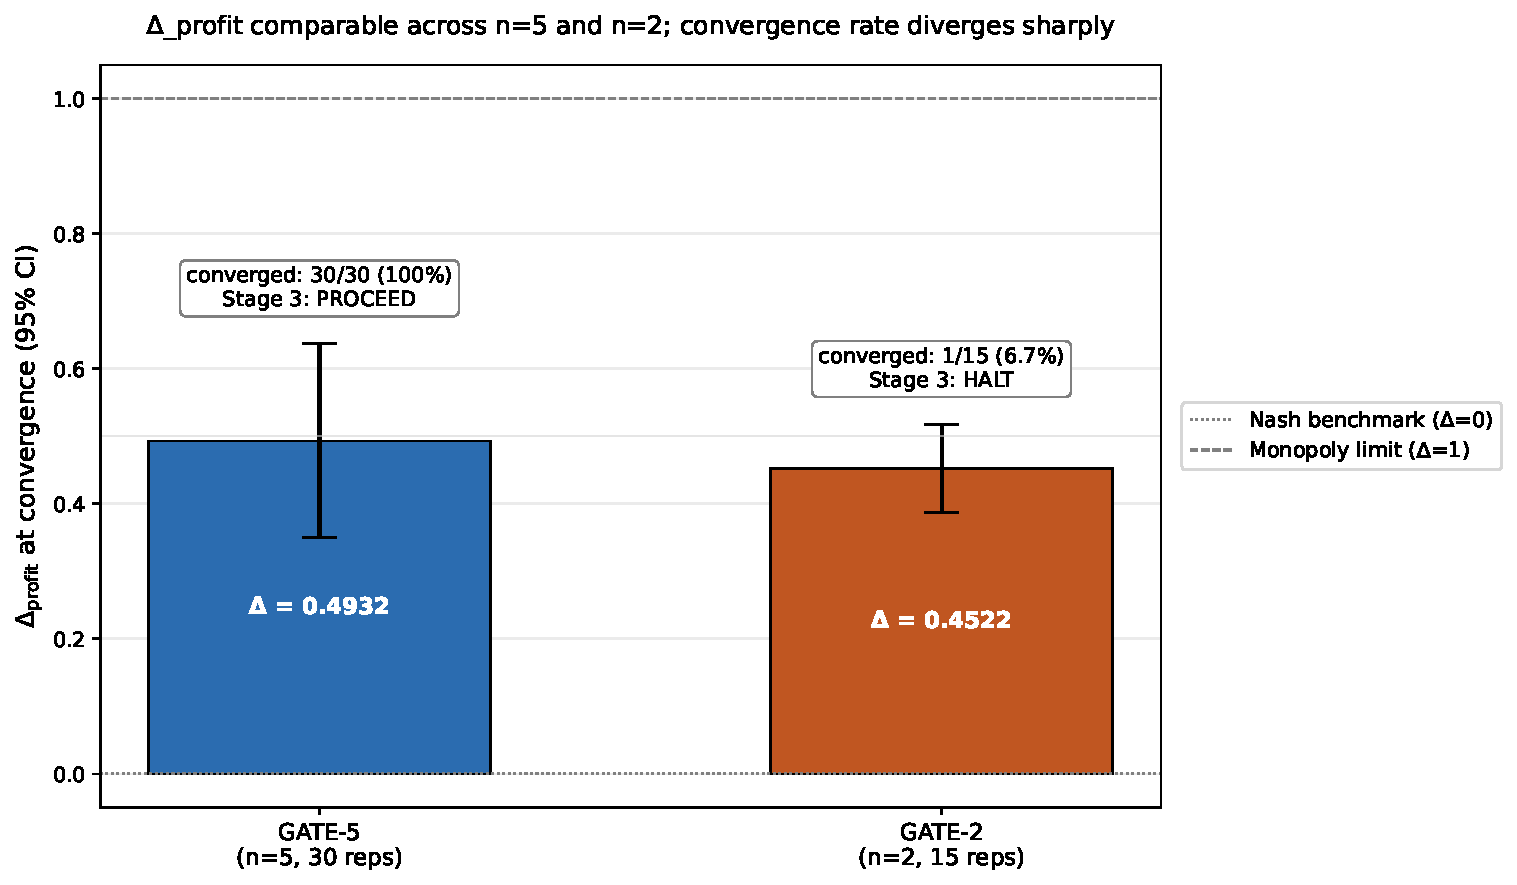
\includegraphics[width=0.95\textwidth]{figures/fig2-delta-profit.pdf}
\caption{$\Delta_{\text{profit}}$ at convergence is comparable across the two conditions ($0.4932$ at $n=5$ vs $0.4522$ at $n=2$), both capturing roughly half of the Nash-to-Monopoly profit gap. The pre-registered Stage 3 go/no-go gate fires PROCEED for GATE-5 and HALT for GATE-2 on convergence-rate grounds, not on $\Delta_{\text{profit}}$ grounds: convergence rate within the 50-round horizon differs sharply ($30/30$ versus $1/15$) and is the asymmetry that anchors this paper. Error bars are 95\% percentile bootstrap CIs ($B = 10{,}000$, fixed seed).}
\label{fig:delta-profit}
\end{figure}

\subsection{Convergence dynamics}
\label{sec:results-convergence}

GATE-5 mean prices settle below the cooperation midpoint $p^{\text{mid}}_5 = 1.7044$ by approximately round 12 (median round of first convergence: 12) and then drift slowly downward through round 50 (round-46 mean $1.605$, round-50 mean $1.558$). GATE-2 mean prices oscillate near the cooperation midpoint $p^{\text{mid}}_2 = 1.6990$ throughout the 50-round horizon, with the window-mean prices over rounds 41--50 ranging $1.606$--$1.640$ --- never settling. The single GATE-2 repetition that satisfies the convergence criterion does so at round 38, which is the latest convergence event in either condition. Figure~\ref{fig:convergence-trajectories} overlays the per-round mean price trajectories for both conditions against the cooperation midpoint and the Nash and Monopoly benchmark levels.

\begin{figure}[h]
\centering
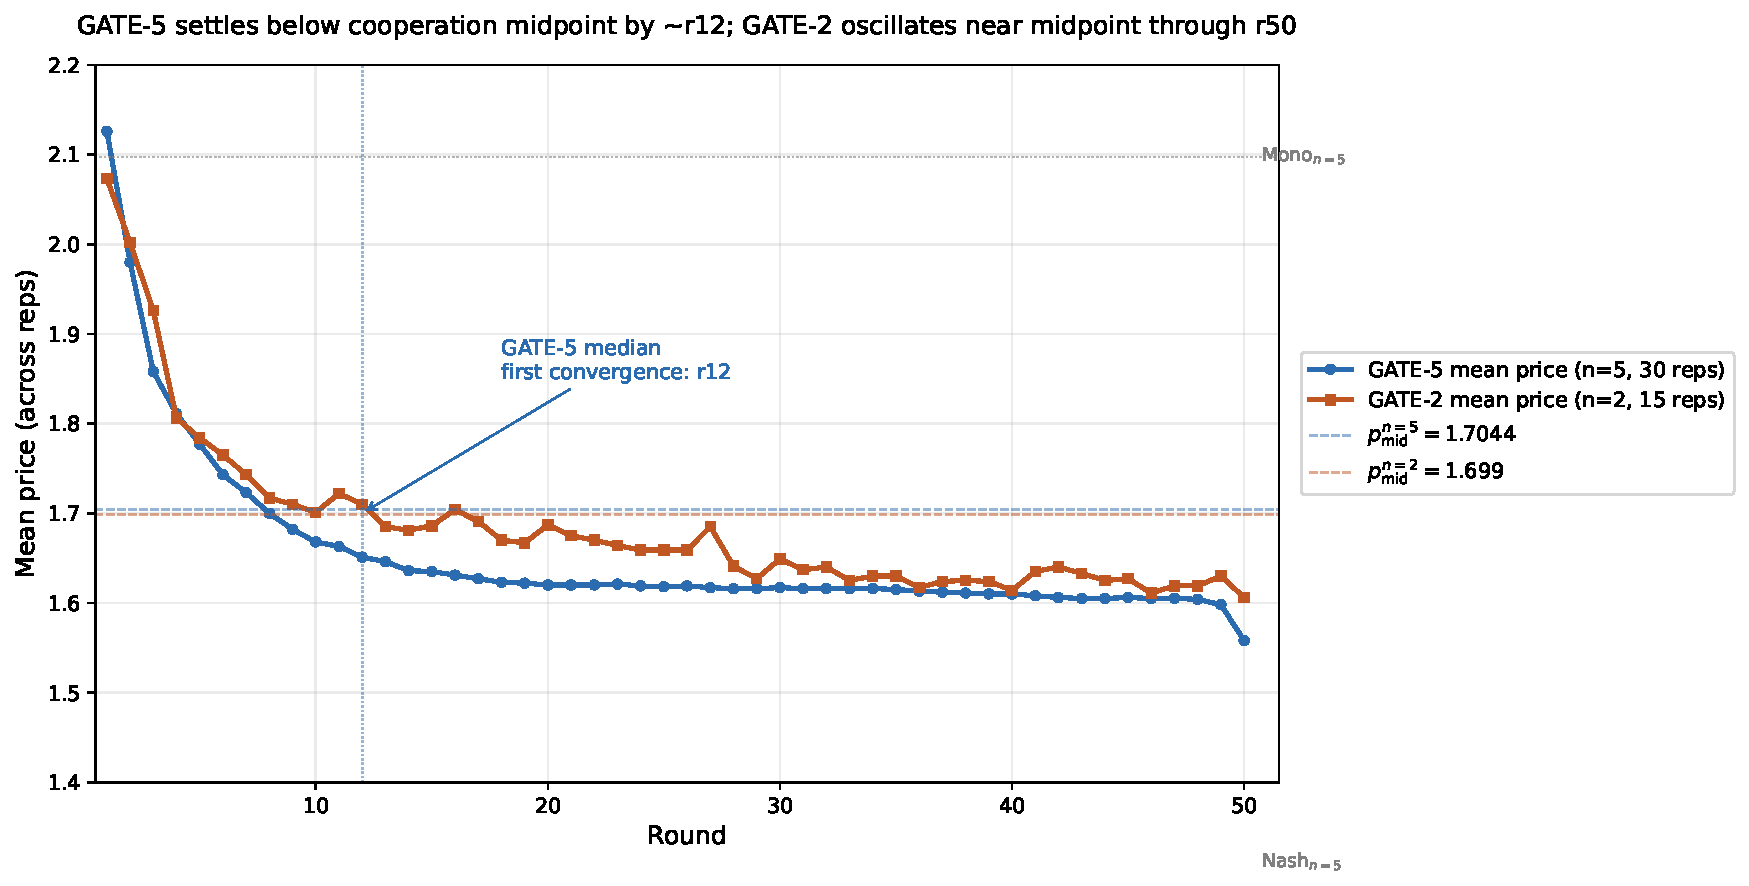
\includegraphics[width=0.95\textwidth]{figures/fig3-convergence-trajectories.pdf}
\caption{Per-round mean price trajectories (averaged across reps) for GATE-5 ($n=5$, 30 reps) and GATE-2 ($n=2$, 15 reps). GATE-5 settles below $p^{\text{mid}}_5 = 1.7044$ by approximately round 12 and drifts slowly downward through round 50; GATE-2 oscillates near $p^{\text{mid}}_2 = 1.6990$ throughout the horizon without settling. The two cooperation midpoints are nearly coincident, so the visual divergence between trajectories reflects basin dynamics, not benchmark differences.}
\label{fig:convergence-trajectories}
\end{figure}

\subsection{Regime classification}
\label{sec:results-regime}

Both conditions are low-regime-dominant. At GATE-5: $8/30$ high ($p_{\text{high}} = 0.267$, Wilson 95\% CI $[0.142, 0.444]$), $0/30$ mid ($p_{\text{mid}} = 0.000$, $[0.000, 0.114]$), $22/30$ low ($p_{\text{low}} = 0.733$, $[0.556, 0.858]$). At GATE-2: $0/15$ high ($p_{\text{high}} = 0.000$, $[0.000, 0.204]$), $4/15$ mid ($p_{\text{mid}} = 0.267$, $[0.109, 0.520]$), $11/15$ low ($p_{\text{low}} = 0.733$, $[0.480, 0.891]$). The pre-registered unimodality null hypothesis ($\max_r p_r \geq 0.80$ with 95\% confidence) is \textbf{not rejected} at either condition: the upper Wilson bound on the dominant low-regime probability is $0.858$ at GATE-5 and $0.891$ at GATE-2.

\subsection{Basin-stability secondary lens}
\label{sec:results-basin}

Per Addendum \#4, each repetition's dominant regime over rounds 31--40 is compared to its dominant regime over rounds 41--50; agreement defines the repetition as basin-stable. Cross-condition basin-stability rates are: GATE-5 $30/30$ ($100.0\%$, Wilson 95\% CI $[0.886, 1.000]$); GATE-2 $12/15$ ($80.0\%$, Wilson 95\% CI $[0.548, 0.930]$). Both conditions clear the pre-registered basin-PROCEED $80\%$ threshold, but the GATE-2 Wilson interval spans the threshold itself: the rate is statistically distinguishable from the $0.50$ baseline (lower bound $0.548 > 0.50$) but the CI is wide enough that the $80\%$ threshold falls inside it --- the basin-PROCEED rule is non-discriminative at $n_{\text{rep}} = 15$ for the duopoly condition; see \S\ref{sec:limitations-envelope} for the cross-result envelope. We acknowledged this single-rep fragility in Methods (\S\ref{sec:methods-sample-size}); it is the primary motivation for the Stage 3 expansion to $n_{\text{rep}} \geq 30$.

\begin{figure}[h]
\centering
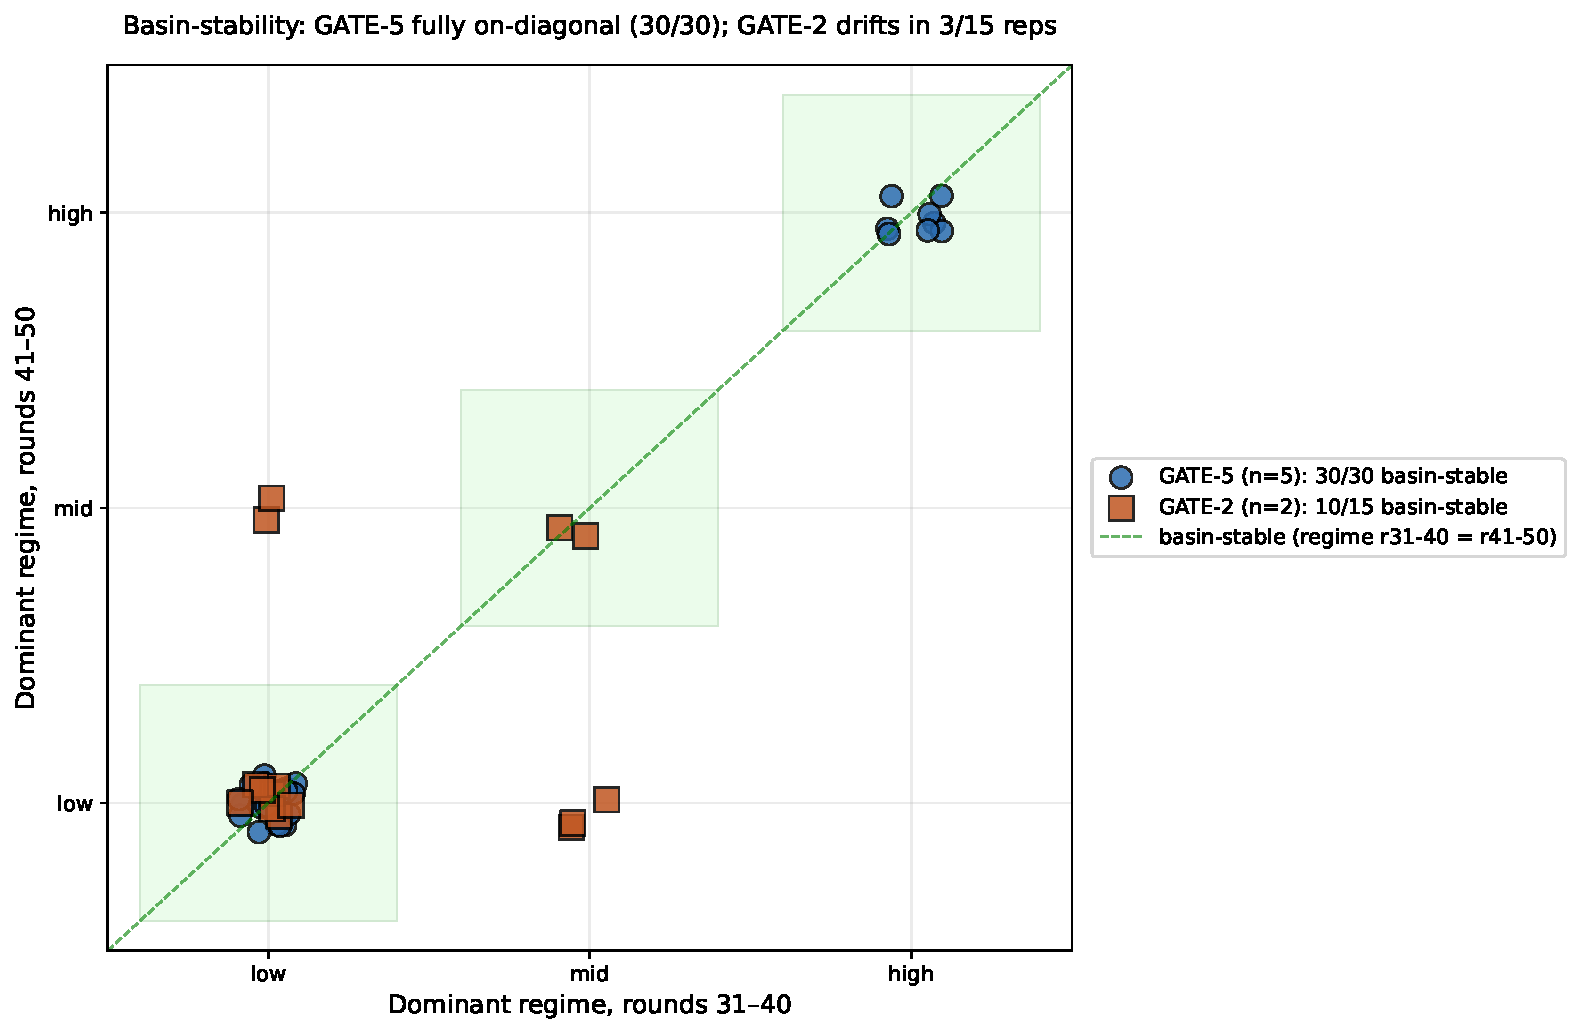
\includegraphics[width=0.95\textwidth]{figures/fig4-basin-stability.pdf}
\caption{Each repetition is plotted at (dominant regime in rounds 31--40, dominant regime in rounds 41--50); on-diagonal points are basin-stable. GATE-5 has $30/30$ reps on the diagonal, with both basins (low $\Delta$ and high $\Delta$) populated. GATE-2 has $12/15$ on the diagonal; the three off-diagonal reps drift from MID in rounds 31--40 to LOW in rounds 41--50, consistent with the wider-basin reading developed in \S\ref{sec:discussion-asymmetry} (mechanism refined in \S\ref{sec:discussion-asymmetry-cot}). The Wilson 95\% CI on the GATE-2 basin-stable rate $[0.548, 0.930]$ spans the basin-PROCEED $0.80$ threshold (the lower bound $0.548$ is above the $0.50$ baseline but the threshold itself sits inside the interval), motivating the Stage 3 expansion.}
\label{fig:basin-stability}
\end{figure}

\subsection{$k$-selection (Addendum \#1 \S A)}
\label{sec:results-kselect}

Bootstrap $k$-selection results are summarized in Table~\ref{tab:k-selection}. At GATE-5, the gap statistic recovers $k = 2$ in $7/10$ resamples (clearing the pre-registered $\geq 7/10$ recovery threshold by exactly one resample); the supplementary 100-resample $\times$ 10-seed sweep (1000 total resamples) yields $k = 2$ in $72.0\%$ aggregated, with $10/10$ seeds returning $k = 2$ as the modal winner --- the locked branch is directionally robust. At GATE-2, the gap statistic recovers $k = 1$ in $10/10$ resamples (and $97.1\%$ aggregated across the supplementary 1000 resamples), unanimously and decisively. BIC over-fits to $k = 5$ in both conditions, which is consistent with known BIC behavior in 1D at small sample sizes; gap statistic is the locked primary, BIC is reported as secondary diagnostic.

\begin{table}[h]
\centering
\caption{Bootstrap $k$-selection (gap-statistic primary, BIC secondary). At GATE-5 the bimodal $k=2$ structure is recovered in $7/10$ resamples (locked branch fires); at GATE-2 the unimodal $k=1$ structure is recovered in $10/10$ resamples (inconclusive branch fires).}
\label{tab:k-selection}
\begin{tabular}{ccccccc}
\toprule
& \multicolumn{5}{c}{Resamples (out of 10) selecting $k$} & \\
\cmidrule(lr){2-6}
Condition & $k=1$ & $k=2$ & $k=3$ & $k=4$ & $k=5$ & Locked branch \\
\midrule
GATE-5 (gap)  & 2  & \textbf{7} & 0 & 0 & 1  & (c) bimodal confirmed \\
GATE-5 (BIC)  & 0  & 0          & 0 & 0 & 10 & --- \\
GATE-2 (gap)  & \textbf{10} & 0 & 0 & 0 & 0 & (d) inconclusive at $n_{\text{rep}}$ \\
GATE-2 (BIC)  & 0  & 2          & 0 & 1 & 7  & --- \\
\bottomrule
\end{tabular}
\end{table}

The pre-committed downgrade clause in Addendum \#1 \S A branch (c) fires at GATE-5: the prior exploratory $k = 4$ quadrimodal narrative is retracted, and the bimodal structure is reported throughout. We retain the exploratory $k = 4$ cluster centroids in the supplementary materials for transparency, but no preprint claim rests on them. At GATE-2, branch (d) fires: $k = 1$ is reported as inconclusive on basin count at this sample size, with interpretation deferred to Stage 3 (or to Stage 4 cross-model replication if the Stage 3 expansion yields a similar outcome).

\subsection{Cluster characterization at GATE-5 $k = 2$}
\label{sec:results-clusters}

Table~\ref{tab:cluster-chars} reports the formal $k = 2$ cluster characterization at GATE-5. Cluster 1 (low-$\Delta$ basin) contains 13 reps with mean $\Delta_{\text{profit}} = +0.0817$; all 13 reside in the low cooperation regime. Cluster 2 (high-$\Delta$ basin) contains 17 reps with mean $\Delta_{\text{profit}} = +0.8078$; this cluster comprises all 8 high-regime reps plus 9 low-regime reps. The high-$\Delta$ basin contains both the high-cooperation reps and a subset of low-cooperation reps that achieve substantial profit gains via partial coordination without crossing the round-level cooperation threshold consistently.

\begin{table}[h]
\centering
\caption{Cluster characterization at the formally selected $k = 2$ (GATE-5). The bimodal split separates a low-$\Delta$ basin around the Nash benchmark from a high-$\Delta$ basin near the monopoly benchmark.}
\label{tab:cluster-chars}
\begin{tabular}{lccccc}
\toprule
Cluster & $n_{\text{rep}}$ & $\bar{\Delta}_{\text{profit}}$ & Mean reasoning (chars) & Mean latency (ms) & Regime composition \\
\midrule
1 (low-$\Delta$ basin)  & 13 & $+0.0817$ & $1234$ & $62{,}303$ & low: 13 \\
2 (high-$\Delta$ basin) & 17 & $+0.8078$ & $1202$ & $52{,}058$ & high: 8, low: 9 \\
\bottomrule
\end{tabular}
\end{table}

\subsection{Reasoning-length correlations}
\label{sec:results-reasoning}

Per the four pre-committed Pearson correlations in Addendum \#1 \S C, with Fisher-$z$ 95\% confidence intervals reported for all four regardless of direction or magnitude:

\begin{itemize}
    \item GATE-5: $r(\text{reasoning}, \Delta_{\text{profit}}) = -0.3027$, Fisher-$z$ 95\% CI $[-0.5978, +0.0646]$ (CI includes 0). $r(\text{latency}, \Delta_{\text{profit}}) = -0.2335$, $[-0.5477, +0.1384]$. $r(\text{reasoning}, \text{latency}) = +0.7797$, $[+0.5833, +0.8900]$ (significant; VIF $= 2.55$). Partial $r(\text{reasoning}, \Delta_{\text{profit}} \mid \text{latency}) = -0.1982$, $[-0.5265, +0.1815]$.
    \item GATE-2: $r(\text{reasoning}, \Delta_{\text{profit}}) = -0.4710$, $[-0.7921, +0.0544]$ (borderline, includes 0). Partial $r(\text{reasoning}, \Delta_{\text{profit}} \mid \text{latency}) = -0.4191$, $[-0.7769, +0.1433]$.
\end{itemize}

At $n_{\text{rep}} = 30$ for GATE-5, the Fisher-$z$ test on the reasoning-length correlation has approximately $39\%$ power to detect a population correlation of $r = -0.30$ at $\alpha = 0.05$; the non-rejection of the pre-registered Wu et al.\ falsification clause (\S\ref{sec:results-wu2025}) is therefore a power-limited consistent-with observation, not a Popperian falsification test. See \S\ref{sec:limitations-envelope} for the cross-result sample-size envelope.

The basin fixed-effects regression of $\Delta_{\text{profit}}$ on reasoning length plus regime dummies (HC3 robust standard errors) returns $\hat{\beta}_{\text{reasoning}} = +6.25 \times 10^{-4}$ at GATE-5 ($p = 0.665$, 95\% CI $[-2.21 \times 10^{-3}, +3.46 \times 10^{-3}]$; basin-high dummy $\hat{\beta} = +0.7096$, $p < 0.001$; $R^2 = 0.573$) and $\hat{\beta}_{\text{reasoning}} = -9.22 \times 10^{-4}$ at GATE-2 ($p = 0.164$). The locked decision rule fires in both conditions: \emph{reasoning length is not statistically distinguishable from zero after basin fixed effects, and is therefore reported as a between-basin discriminator candidate, not a within-basin signature.}

\subsection{Cluster-level reasoning-length effect size}
\label{sec:results-cluster-effect}

Under the strict effect-size + confidence-interval test specified in the supplementary materials (\texttt{2026-04-27-addendum1-supplementary-N2-N3.md} \S 12), the cluster-mean reasoning-length difference at the formally selected GATE-5 $k = 2$ is descriptively present with a medium effect size but the 95\% CIs span zero. The low-$\Delta$ basin (cluster 1, $n = 13$) exhibits mean reasoning length $1233.75$ chars (SD $51.16$); the high-$\Delta$ basin (cluster 2, $n = 17$) exhibits $1201.80$ chars (SD $54.09$). The mean difference is $+31.95$ chars ($+2.66\%$ relative), with Cohen's $d = +0.6044$ (medium effect; Hedges' $g = +0.5881$). Welch's $t$-test returns $t(26.7) = +1.6532$, $p = 0.110$, with 95\% CI on the mean difference $[-7.73, +71.62]$ chars; bootstrap percentile 95\% CI $[-4.60, +68.13]$; bootstrap BCa 95\% CI $[-6.64, +66.74]$.

\textbf{Locked downgrade:} the between-basin pattern is descriptively present with a medium effect size, but we do not claim formal between-basin discrimination at this sample size; see \S\ref{sec:limitations-envelope} for the cross-result envelope. The direction is consistent with the Wu et al.\ 2025 simplicity-bias prediction (cluster 1 low-$\Delta$ basin reasons more than cluster 2 high-$\Delta$ basin); Stage 4 cross-model replication is the formal test.

\subsection{Per-host descriptives and host-effect test}
\label{sec:results-host}

The n=15 GATE-2 dataset is split across two host machines after the Addendum \#4 \S C2 trace-integrity rejection of one host's slice (rejected for multi-run trace concatenation; rejection event documented in Addendum \#4 \S C2 at \texttt{pilot/admin/osf-stage2b-addendum-2026-04-26.md} and the per-host audit at \texttt{pilot/admin/team-notes/2026-04-26-host-effect-analysis.md} \S A). Per-host descriptives are reported in Table~\ref{tab:host-descriptives}.

\begin{table}[h]
\centering
\caption{Per-host descriptive statistics at GATE-2 ($n_{\text{rep}} = 15$, split 10/5 across two host machines).}
\label{tab:host-descriptives}
\begin{tabular}{lcccccc}
\toprule
Host & Reps & $\bar{\Delta}_{\text{profit}}$ & 95\% CI ($B = 10^4$) & Regime H/M/L & Converged & Mean wall-clock (s) \\
\midrule
Host A & 10 & $0.4018$ & $[0.3203, 0.4696]$ & 0/1/9  & 0/10 & 3499.1 \\
Host B & 5  & $0.5530$ & $[0.5200, 0.5945]$ & 0/3/2  & 1/5  & 2589.5 \\
\bottomrule
\end{tabular}
\end{table}

The two-tailed Fisher's exact host-effect test on the regime $\times$ host contingency (effective $2 \times 2$ over MID/LOW $\times$ Host A/Host B; HIGH regime is empty in this dataset) returns $p = 0.0769$ with odds ratio $13.500$. Per the pre-committed Addendum \#3 \S B2 decision rule for $p \geq 0.05$, the data are consistent with no host effect within the power of the test, but a meaningful host effect cannot be ruled out at $n_{\text{rep}} = 15$ split 10/5; see \S\ref{sec:limitations-envelope} for the cross-result envelope. Stage 3 expansion to $n_{\text{rep}} \geq 30$ is required before any equivalence claim is appropriate.

\paragraph{Within-Host-A pairwise temporal-stability check.}
Host A's 10 repetitions are split across two non-contiguous wall-clock windows separated by approximately 24 hours on the same machine (slice 1: 5 reps on 2026-04-24; slice 2: 5 reps on 2026-04-25). Pairing rep $i$ in slice 1 with rep $i$ in slice 2 by within-host index, the pairwise regime match rate is $4/5 = 80.0\%$ (Wilson 95\% CI $[0.376, 0.964]$; Figure~\ref{fig:host-pairwise}). The single discordant pair is rep 2 (slice 1: mid, $\Delta = 0.4364$, coop $= 0.200$) versus its slice-2 counterpart (low, $\Delta = 0.1502$, coop $= 0.050$); a $0.150$ cooperation drift just clears the $0.20$ MID/LOW classifier boundary. We report $4/5$ as the primary within-Host-A statistic; the $n = 5$ pairs is too small for a formal test, so this rate is reported descriptively. The corresponding Fisher's exact on the within-Host-A $2 \times 2$ MID/LOW $\times$ slice contingency is degenerate (zero cell $d = 0$ in slice 2; the observed table is the most extreme under the null, forcing $p = 1.0000$ and $\text{OR} = 0.000$); we report this Fisher's value for transparency only and do not interpret it as evidence of distributional equivalence.

\begin{figure}[h]
\centering
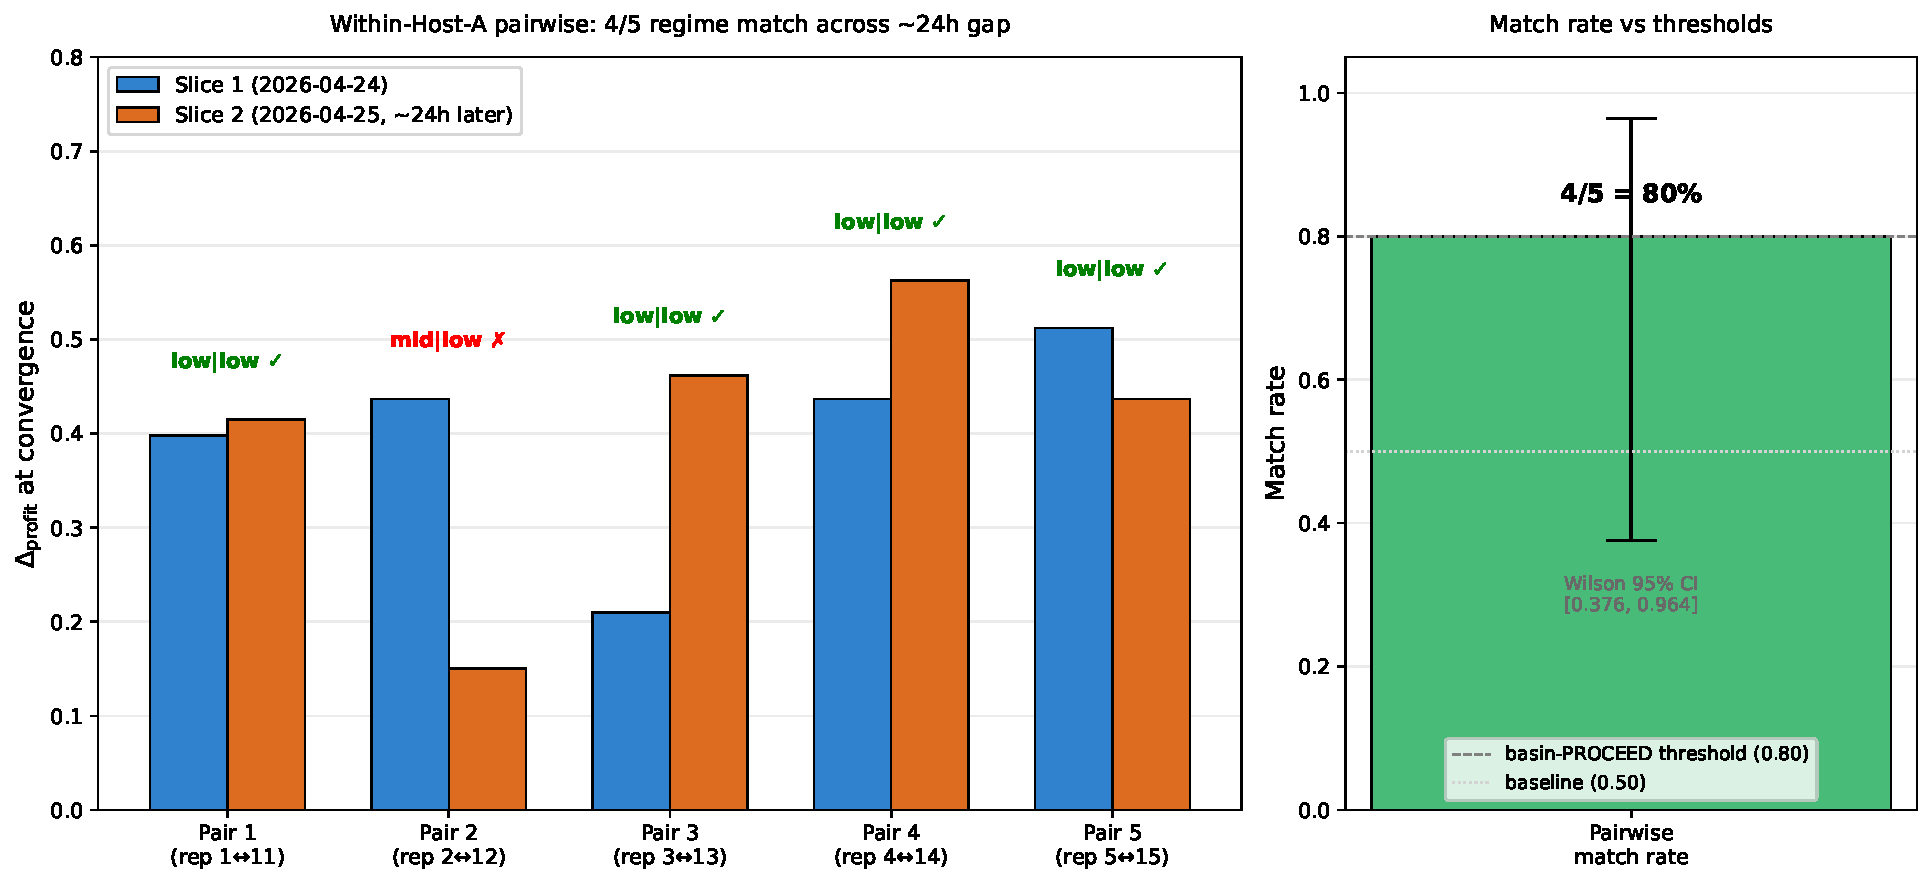
\includegraphics[width=0.95\textwidth]{figures/fig5-host-pairwise.pdf}
\caption{Within-Host-A pairwise temporal-stability check: 5 repetition pairs spanning a $\sim 24$-hour gap on the same machine. Left: per-pair $\Delta_{\text{profit}}$ in slice 1 (2026-04-24) versus slice 2 (2026-04-25), with regime labels and match indicator above each pair. Right: pairwise regime match rate $4/5 = 80\%$ with Wilson 95\% CI $[0.376, 0.964]$; the CI overlaps both the basin-PROCEED $0.80$ threshold and the $0.50$ baseline, so the $80\%$ rate is reported as descriptive consistency evidence per Revision D --- the $n = 5$ pairs is too small for a formal equivalence test. The single discordant pair (rep 2 vs rep 12) reflects a $0.150$ cooperation drift just clearing the MID/LOW classifier boundary.}
\label{fig:host-pairwise}
\end{figure}

\subsection{Survivor-rep consistency}
\label{sec:results-survivor}

The survivor-rep consistency check operates on $n = 4$ reps total (2 survivor reps from a 2026-04-23 ratelimit-failed pilot, plus 2 re-run reps from the canonical 2026-04-24 slice). The verdict is \textbf{consistency-negative} on the regime-label dimension: survivor rep 1 (mid, coop $0.450$) versus re-run rep 1 (low, coop $0.150$); survivor rep 2 (low, coop $0.150$) versus re-run rep 2 (mid, coop $0.200$). However, the underlying numerics are tight across all four reps: $\Delta_{\text{profit}}$ at convergence ranges $0.40$--$0.51$, mean price ranges $1.598$--$1.638$ (all within $\pm 0.04$ of the cooperation midpoint $1.6990$), chain-of-thought length ranges $1209$--$1237$ chars, parse success $100\%$ across all four.

The mechanism interpretation is round-level threshold sensitivity, not a $0.20$ MID/LOW classifier-boundary artifact. Per-round cooperation labels are computed as $\mathbb{1}[\bar{p}_t > p^{\text{mid}}_2 = 1.6990]$, and the survivor and re-run reps both have window-mean prices oscillating in the $1.598$--$1.638$ range --- within $\pm 0.04$ of the midpoint. Small per-round price drift flips many round-level cooperation labels, which propagates noisily to the rounds 41--50 regime aggregate. The substantive drift at survivor rep 1 (coop $0.450 \to 0.150$, $\Delta = 0.300$) is not at the $0.20$ classifier boundary; it is a round-level threshold-sensitivity artifact that aggregates upward to the regime label. $n = 4$ is too small to formally distinguish threshold-aggregation noise from substantive drift; we frame this exploratorily and defer mechanism adjudication to Stage 4 cross-model replication.

\subsection{Wu et al.\ 2025 simplicity-bias falsifiability test}
\label{sec:results-wu2025}

Per the pre-registered Addendum \#1 \S D falsifiability clause, the Wu et al.\ 2025 simplicity-bias mechanism predicts shorter chain-of-thought reasoning at more-cooperative basins (if the cooperative-pricing answer is representationally simpler for a Haiku-class pretrained agent, simplicity-bias predicts shorter reasoning at higher $\Delta_{\text{profit}}$). The falsification clause is: \emph{$r(\text{reasoning length}, \Delta_{\text{profit}}) > 0$ at GATE-5 falsifies simplicity-bias as the operative mechanism.} The point-estimate signs at both agent counts are consistent with the prediction ($r = -0.30$ at $n = 5$, $r = -0.47$ at $n = 2$), but Fisher-$z$ 95\% confidence intervals span zero in both conditions; see \S\ref{sec:limitations-envelope} for the cross-result envelope. The pre-registered falsification clause is \textbf{not triggered} (the GATE-5 point estimate is negative); the mechanism is consistent with the data direction but is not strongly confirmed at this sample size. The pre-committed Stage 4 cross-model replication (across Haiku sizes, Sonnet, Opus, and non-Anthropic frontier models) is the formal falsification test.

\subsection{Verification outcome}
\label{sec:results-verification}

The independent Python/SciPy reference verifier (\texttt{verify-stage2b-2026-04-26.py}, \texttt{verify-formalize-2026-04-26.py}) returns \texttt{ALL CLAIMS REPRODUCE: True} across all six pre-registered claim categories (Calvano benchmark prices, per-rep $\Delta_{\text{profit}}$ values and CIs, Stage 3 verdicts, basin-stability counts, drift directions, asymmetry-finding numerics) and across all formalized Addendum \#1 statistical operations (Pearson $r$ at $|\Delta| < 10^{-4}$, Fisher-$z$ CI bounds at $|\Delta| < 10^{-4}$, VIFs at $|\Delta| < 10^{-4}$, full-sample gap-statistic $k$ exact, bootstrap $k$-selection identical under matched seed). The bug surfaced and fixed by the cross-toolchain procedure (Fisher's exact denominator error in \texttt{pilot/analyze-host-effect.ts}; \S\ref{sec:methods-rigor}) is the only correction required to the headline analyses prior to this preprint.
